\documentclass[12pt,]{article}
\usepackage[left=1in,top=1in,right=1in,bottom=1in]{geometry}
\newcommand*{\authorfont}{\fontfamily{phv}\selectfont}
\usepackage[]{mathpazo}


  \usepackage[T1]{fontenc}
  \usepackage[utf8]{inputenc}




\usepackage{abstract}
\renewcommand{\abstractname}{}    % clear the title
\renewcommand{\absnamepos}{empty} % originally center

\renewenvironment{abstract}
 {{%
    \setlength{\leftmargin}{0mm}
    \setlength{\rightmargin}{\leftmargin}%
  }%
  \relax}
 {\endlist}

\makeatletter
\def\@maketitle{%
  \newpage
%  \null
%  \vskip 2em%
%  \begin{center}%
  \let \footnote \thanks
    {\fontsize{18}{20}\selectfont\raggedright  \setlength{\parindent}{0pt} \@title \par}%
}
%\fi
\makeatother




\setcounter{secnumdepth}{0}

\usepackage{longtable,booktabs}



\title{Effects of macronutrient manipulation in artificial diet on fall
armyworm (\emph{Spodoptera frugiperda}) performance  }
 



\author{\Large Kale
Costanza\vspace{0.05in} \newline\normalsize\emph{Department of
Biological Sciences, Louisiana State University, Baton Rouge, Louisiana,
USA \textbar{} 232 Life Sciences Building \textbar{}
\href{mailto:kcosta3@lsu.edu}{\nolinkurl{kcosta3@lsu.edu}}}  }


\date{}

\usepackage{titlesec}

\titleformat*{\section}{\normalsize\bfseries}
\titleformat*{\subsection}{\normalsize\itshape}
\titleformat*{\subsubsection}{\normalsize\itshape}
\titleformat*{\paragraph}{\normalsize\itshape}
\titleformat*{\subparagraph}{\normalsize\itshape}



\usepackage{biblatex}

\addbibresource{ref.bib}


\newtheorem{hypothesis}{Hypothesis}
\usepackage{setspace}


% set default figure placement to htbp
\makeatletter
\def\fps@figure{htbp}
\makeatother

\usepackage{indentfirst}
\usepackage{graphicx}
\graphicspath{ {images/} }
\usepackage{float}

% move the hyperref stuff down here, after header-includes, to allow for - \usepackage{hyperref}

\makeatletter
\@ifpackageloaded{hyperref}{}{%
\ifxetex
  \PassOptionsToPackage{hyphens}{url}\usepackage[setpagesize=false, % page size defined by xetex
              unicode=false, % unicode breaks when used with xetex
              xetex]{hyperref}
\else
  \PassOptionsToPackage{hyphens}{url}\usepackage[draft,unicode=true]{hyperref}
\fi
}

\@ifpackageloaded{color}{
    \PassOptionsToPackage{usenames,dvipsnames}{color}
}{%
    \usepackage[usenames,dvipsnames]{color}
}
\makeatother
\hypersetup{breaklinks=true,
            bookmarks=true,
            pdfauthor={Kale Costanza (Department of Biological Sciences,
Louisiana State University, Baton Rouge, Louisiana, USA \textbar{} 232
Life Sciences Building \textbar{}
\href{mailto:kcosta3@lsu.edu}{\nolinkurl{kcosta3@lsu.edu}})},
             pdfkeywords = {fall armyworm, \emph{Spodoptera frugiperda},
resource quality, climate change},  
            pdftitle={Effects of macronutrient manipulation in
artificial diet on fall armyworm (\emph{Spodoptera frugiperda})
performance},
            colorlinks=true,
            citecolor=blue,
            urlcolor=blue,
            linkcolor=magenta,
            pdfborder={0 0 0}}
\urlstyle{same}  % don't use monospace font for urls

% Add an option for endnotes. -----


% add tightlist ----------
\providecommand{\tightlist}{%
\setlength{\itemsep}{0pt}\setlength{\parskip}{0pt}}

% add some other packages ----------

% \usepackage{multicol}
% This should regulate where figures float
% See: https://tex.stackexchange.com/questions/2275/keeping-tables-figures-close-to-where-they-are-mentioned
\usepackage[section]{placeins}


\begin{document}
	
% \pagenumbering{arabic}% resets `page` counter to 1 
%    

% \maketitle

{% \usefont{T1}{pnc}{m}{n}
\setlength{\parindent}{0pt}
\thispagestyle{plain}
{\fontsize{18}{20}\selectfont\raggedright 
\maketitle  % title \par  

}

{
   \vskip 13.5pt\relax \normalsize\fontsize{11}{12} 
\textbf{\authorfont Kale Costanza} \hskip 15pt \emph{\small Department
of Biological Sciences, Louisiana State University, Baton Rouge,
Louisiana, USA \textbar{} 232 Life Sciences Building \textbar{}
\href{mailto:kcosta3@lsu.edu}{\nolinkurl{kcosta3@lsu.edu}}}   

}

}








\begin{abstract}

    \hbox{\vrule height .2pt width 39.14pc}

    \vskip 8.5pt % \small 

\noindent As global climate change raises atmospheric carbon dioxide
levels, this can lead to increased carbon sequestration in plants and
consequential nutrient dilution in resources for insect herbivores. The
fall armyworm (\emph{Spodoptera frugiperda}) is an invasive agricultural
pest that may experience drastic changes in performance and development
as a result of such resource quality variation. In this experiment, I
manipulated the protein-to-carbohydrate (P:C) ratios in artificial diet
treatments to investigate potential effects of macronutrient
manipulation on fall armyworm development. I found that high
carbohydrate levels, relative to protein (1:5, C diet), yielded very low
survival and no chance of pupation. Equal P:C levels (1:1, B) or even
higher protein (5:1, A) allowed for pupation, but this was only
successful when larvae were placed on manipulated diet at the third
instar as opposed to first instar. A and B diets were usually found to
be statistically similar in terms of pupation qualities (age and mass),
but overall trends of development were noticeably different for all
three (A, B, C) manipulated diet treatments. My results suggest that
there are key differences in performance depending on the nutritional
composition fed to the larvae. I believe that feeding these same diet
formulas for a shorter portion of the lifespan will be helpful to then
run further experimental tests, such as investigating the combined
effects of resource quality and temperature variation on cannibalism and
disease transmission.


\vskip 8.5pt \noindent \emph{Keywords}: fall armyworm, \emph{Spodoptera
frugiperda}, resource quality, climate change \par

    \hbox{\vrule height .2pt width 39.14pc}



\end{abstract}


\vskip -8.5pt


 % removetitleabstract

\noindent  

\hypertarget{introduction}{%
\section{Introduction}\label{introduction}}

Global climate change is a major topic of concern for modern ecologists.
Worldwide average temperature changes are likely to impact the behavior
and distribution of many insect species; for those with unique
host-pathogen systems, disease transmission may change as a result
\autocite{elderd_warmer_2014}. Rising atmospheric carbon dioxide may
lead to increased plant biomass and consequential nutrient dilution in
resources for insect herbivores \autocite{welti_nutrient_2020}. As
carbon increases in plant material, the nitrogen-to-carbon ratio
decreases, ultimately diluting the amount of protein consumed compared
to carbohydrates \autocite{shikano_impact_2015}.

For the fall armyworm (\emph{Spodoptera frugiperda}; ``FAW''), such
changes in temperature and resource quality are likely to alter the
insect's overall performance and development. The fall armyworm is a
moth species of the Noctuidae family; during its larval stage, it acts
as a ravenous herbivore that prefers grasses but will consume a wide
range of vegetation. The FAW is a prominent agricultural pest in its
native regions of North and South America and acts as a devastating
invasive species to other continents where it has been introduced
\autocite{noauthor_spodoptera_nodate}. It primarily attacks crops such
as corn/maize, soybeans, sorghum, wheat, and others.

The fall armyworm has a specialist baculovirus, the \emph{Spodoptera
frugiperda} multiple nucleopolyhedrovirus (SfMNPV), that is both
naturally occurring and used as a biopesticide. Fall armyworms are
frequently cannibalistic in their larval stage, an important mode of
baculovirus transmission \autocite{valicente_cannibalism_2013}. When
competing for scarce resources, FAW larvae are more likely to
cannibalize their conspecifics to gain nutritional benefit
\autocite{ren_functional_2020}. As resource quality diminishes and
temperatures rise, it is possible that FAW larvae will increase
cannibalism of conspecifics and therefore increase baculovirus
transmission.

As a first step to exploring potential effects of climate change on this
system, it is necessary to explore how varying resource quality --- most
notably the protein:carbohydrate ratio --- may impact the performance of
the fall armyworm. In this paper, I will describe my experimental
testing of resource quality on fall armyworm performance and its
connection to the broader subject of climate change and disease
transmission.

\hypertarget{methods-materials}{%
\section{Methods \& Materials}\label{methods-materials}}

\hypertarget{faw-larvae-source}{%
\subsection{\texorpdfstring{\textbf{FAW Larvae
Source}}{FAW Larvae Source}}\label{faw-larvae-source}}

Fall armyworm larvae were sourced from Dr.~Bret Elderd's
laboratory-reared colony. The colony originated from wild-caught
individuals (F0) from corn fields around Purdue University in West
Lafayette, Indiana, USA. This ``Purdue'' colony was reared for a
long-term coevolution project, including one line kept at 26°C during
the day and 16°C at night that was infected each generation with a 50\%
lethal dose of SfMNPV (``26/16 coevolved line''). I used new
first-instar larvae from this particular colony line (F17) for my
experiment. Fall armyworms have a total of six larval instars before the
pupal stage.

\hypertarget{artificial-diet-treatments}{%
\subsection{\texorpdfstring{\textbf{Artificial Diet
Treatments}}{Artificial Diet Treatments}}\label{artificial-diet-treatments}}

There are four total artificial diet treatments used in this experiment,
including three macronutrient-manipulated formulas (``manipulated''
diets) and one premade standard formula (``control'' diet). The control
diet is produced and sold by Southland Products, Inc.~(``Southland
diet'') \autocite{noauthor_southland_nodate} and is the typical diet fed
to colony FAWs in Dr.~Bret Elderd's lab, where these larvae were
sourced.

I based my macronutrient ratios on experimental diet treatments
described in the Shikano and Cory 2015 \autocite{shikano_impact_2015}
paper on cabbage loopers, a similar Noctuid moth to the fall armyworm.
While their protein:carbohydrate ratios were based on the cabbage
looper's preferred host plant (\emph{Brassicacae} species), the range is
sufficient for fall armyworms as well; soybean plants, which are readily
eaten by fall armyworms and used in Elderd lab research, have a dry
composition of roughly 30\% protein and 30\% carbohydrates
\autocite{wrigley_encyclopedia_2004}. I sourced the original diet recipe
directly from Dr.~Ikkei Shikano with slight modifications. Casein
(protein) and sucrose (carbohydrate) compose 60\% of the total dry
weight in all manipulated diets, with the ratio of each
(protein:carbohydrate) changing depending on the treatment assigned (A =
50\%:10\% or 5:1, B = 30\%:30\% or 1:1, C = 10\%:50\% or 1:5). The
remaining 40\% of dry ingredients are as follows: cellulose (25\%),
cholesterol (1.5\%), Wesson salt (5\%), ascorbic acid (1\%), sorbic acid
(0.5\%), sodium alginate (2.5\%), Vanderzant vitamin mix (3.5\%), and
linseed oil (1\%). Southland (control) diet has a reported dry
nutritional composition of 23.5\% protein and 57\% carbs (\(\approx\)
1:2.5 P:C ratio).

To prepare the A, B, and C treatment diets, dry ingredients were
combined with room temperature water (volume = total dry mass x 2.67)
and blended thoroughly. Agar (mass = total dry mass x .0675) was
dissolved completely in boiling water (volume = total dry mass x 2.33)
and then poured into the same blender. This gives a dry-to-wet mass
ratio of \(\approx\) 1:5. The mixture was blended on high for two
minutes. The liquid diet was poured into 1-oz. plastic cups until about
a quarter filled then allowed to completely cool and solidify. Diet was
stored in a refrigerator at 4°C until use. Jin et al.~2020 was very
helpful in my understanding of the physical preparation process for fall
armyworm artificial diet \autocite{jin_comparative_2020}.

\hypertarget{experimental-setup}{%
\subsection{\texorpdfstring{\textbf{Experimental
Setup}}{Experimental Setup}}\label{experimental-setup}}

Thirty individual larvae were placed into each of the following
treatments: Control, A at First Instar, A at Third Instar, B at First
Instar, B at Third Instar, C at First Instar, and C at Third Instar (N =
210 total; 30 per unique diet/age treatment). Larvae were taken at first
instar from hatching bags and individually placed into a (room
temperature) 1-oz. cup of their respective diet. Control larvae were
kept on Southland diet the whole time; A/B/C at First Instar larvae were
placed on their respective diet immediately; A/B/C at Third Instar
larvae were initially placed on Southland diet and individually
transferred to their assigned diet as soon as they molted into an early
third instar. All larvae were kept at a standard 31°C/21°C
daytime/nighttime (14 hours/10 hours) temperature schedule in Conviron
brand incubators.

After initial setup, each individual larva was checked daily for
mortality and instar status. If it molted into a new instar or died, the
date was recorded for that event. If it successfully pupated, the date
was recorded and the pupa had its mass measured in milligrams on a
precision scale and its sex identified under a dissecting scope. If any
pupae eclosed as moths, the date was recorded and so was the moth's
status --- either healthy, non-functional wings/deformed, or failed to
fully emerge. Monitoring continued until all individuals had either died
or become moths.

\hypertarget{data-analysis}{%
\subsection{\texorpdfstring{\textbf{Data
Analysis}}{Data Analysis}}\label{data-analysis}}

In order to evaluate performance of these fall armyworms fed various
diets, I focused on measures of pupation (end of diet consumption ---
successful outcome) and larval mortality (death as a larva ---
unsuccessful outcome). I completed all data analysis in R version 4.3.1
\autocite{r_core_team_r_2023}.

\hypertarget{pupation}{%
\subsubsection{Pupation}\label{pupation}}

For measures of pupation, I looked at pupation success rates, time to
pupation, and pupal mass. I summarized the total number of successful
pupae and moths for each treatment, as displayed in a bar graph. Using
base R functions, I created histograms for overall time to pupation for
all treatments that produced pupae; this measured total days from first
instar until pupal stage. I then performed an ANOVA, Tukey test, and
t-tests on the most relevant pupae data to determine significant
differences between treatment groups. I did the same analyses --- ANOVA,
Tukey test, and t-tests --- to check for significant differences in mean
pupal mass between treatments and created a boxplot (\emph{ggplot2} R
package \autocite{wickham_ggplot2_2016}) to visualize the data.

\hypertarget{mortality}{%
\subsubsection{Mortality}\label{mortality}}

To analyze larval mortality, I used the \emph{survival} R package
\autocite{therneau_package_2023,bos_ants_2015} to perform a survival
analysis, as well as \emph{ggplot2} \autocite{wickham_ggplot2_2016},
\emph{ggsurvfit} \autocite{sjoberg_ggsurvfit_2023}, and \emph{survminer}
\autocite{kassambara_survminer_2021} packages to visualize the results.
I used a survival regression model (\emph{survreg} function) and did a
chi-square test on mortality between treatments.

\hypertarget{results}{%
\section{Results}\label{results}}

\hypertarget{pupation-1}{%
\subsubsection{Pupation}\label{pupation-1}}

Individuals pupated successfully in the A at Third Instar (``A3rd''), B
at First Instar (``B1st''), B at Third Instar (``B3rd''), and Control
groups, as shown in Figure 1. Most Control group individuals (26 out of
30) pupated, while only 11 of 30 individuals in the A3rd group pupated,
2 in the B1st group, and 3 in the B3rd group.

\begin{figure}

{\centering 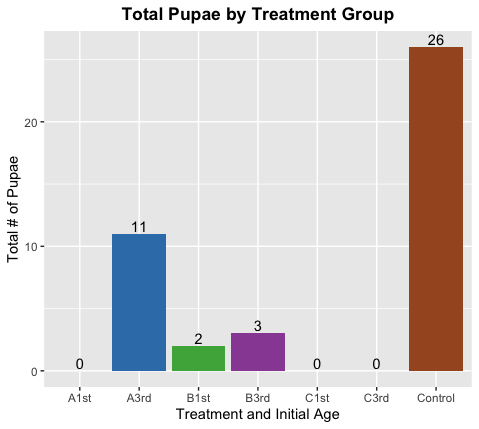
\includegraphics[width=0.5\linewidth]{../Figures/Figure_1} 

}

\caption{Total number of individuals that pupated per treatment group (type of diet and initial age).}\label{fig:Figure1}
\end{figure}

All other individuals died during one of their larval instars. 25 of the
26 Control pupae successfully emerged as a moth (either healthy or with
deformed wings) and 1 of the A3rd group pupae attempted to eclose but
did not succeed. No other pupae became moths.

The overall time to pupation (in days from first instar to pupation) is
visualized as a histogram in Figure 2. See Table 1 for a summary of
pupation values.

Table 1: Number of pupae and mean, fastest, and slowest times to
pupation for each group. Time is given in days from first instar to
pupation.

\begin{longtable}[]{@{}lllll@{}}
\toprule\noalign{}
Treatment Group & \# Pupae & Mean Time & Fastest & Slowest \\
\midrule\noalign{}
\endhead
\bottomrule\noalign{}
\endlastfoot
Control & 26 & 14.7 & 13 & 17 \\
A3rd & 11 & 18.7 & 15 & 22 \\
B1st & 2 & 21 & 20 & 22 \\
B3rd & 3 & 17.3 & 16 & 18 \\
\end{longtable}

\begin{figure}

{\centering 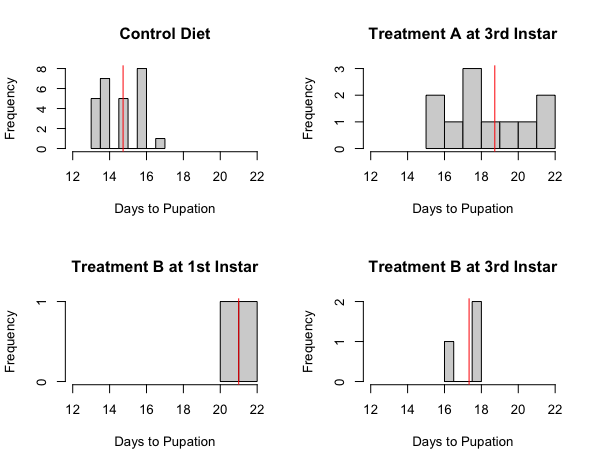
\includegraphics[width=0.75\linewidth]{../Figures/Figure_2} 

}

\caption{Histograms of total days to pupation for all relevant treatments. This only includes the treatments that produced pupae (Control, A at Third Instar, B at First Instar, and B at Third Instar). Here, time to pupation is being measured as days from first instar until pupal stage. The vertical red lines represent the mean time to pupation for each treatment.}\label{fig:Figure2}
\end{figure}

Considering the absence of pupae from most treatments started at first
instar, I further statistically analyzed only the treatments that
started at third instar and controls. For consistency, I examined only
the time in pupation from start of third instar until pupal stage. I
created a linear regression model of this data subset and used an ANOVA
to analyze variance between the means of each group. The ANOVA yielded
\(p = 2.737e-08\), which is highly significant (\(p < 0.05\)). I then
ran a Tukey test to determine pairwise specifics, which showed
significant differences between the Control group and A3rd treatment
(\(p = 2.408e-08\)), as well as between the Control group and B3rd
treatment (\(p = 1.365e-02\)). The difference between A3rd and B3rd
groups was not significant (\(p = 0.404\)) according to the Tukey test.
I ran individual t-tests comparing each group as pairs and found that
the results for Control vs.~A3rd were corroborated (\(p = 7.636e-05\));
the Control vs.~B3rd group results were considered not statistically
significant here, although the value is close (\(p = 0.0863\)). The
result for A3rd vs.~B3rd was corroborated here as well (\(p = 0.312\)).

Since pupal mass is linked to reproductive fitness
\autocite{garvey_examining_2022}, it is important to evaluate pupal
masses between treatment groups as well. A boxplot of pupal masses is
given in Figure 3; this shows the median values, interquartile ranges,
minimums, and maximums for each group. See Table 2 for a summary of
pupal masses.

\begin{figure}

{\centering 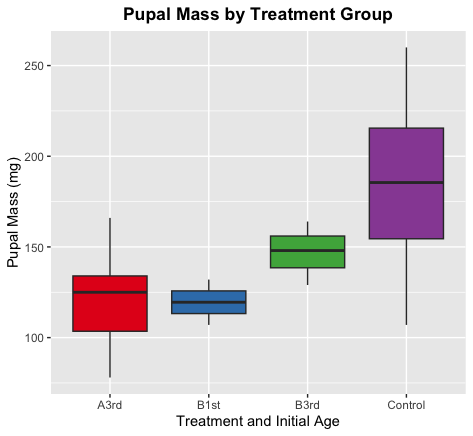
\includegraphics[width=0.5\linewidth]{../Figures/Figure_3} 

}

\caption{Boxplot of pupal mass (in milligrams) for each treatment group (type of diet and initial age) that produced pupae.}\label{fig:Figure3}
\end{figure}

Table 2: Number of pupae and mean, heaviest, and lightest pupal masses
for each group. Mass is measured in milligrams.

\begin{longtable}[]{@{}lllll@{}}
\toprule\noalign{}
Treatment Group & \# Pupae & Mean Mass & Heaviest & Lightest \\
\midrule\noalign{}
\endhead
\bottomrule\noalign{}
\endlastfoot
Control & 26 & 181.8 & 260 & 107 \\
A3rd & 11 & 122.3 & 166 & 78 \\
B1st & 2 & 119.5 & 132 & 107 \\
B3rd & 3 & 147 & 164 & 129 \\
\end{longtable}

I used a linear regression model for pupal mass data and ran an ANOVA
here as well. The ANOVA was significant with \(p = 6.254e-4\).
Performing a Tukey test, however, revealed that the only comparison with
a significant difference is the Control vs.~A3rd pair (\(p = 7.10e-4\)).
All other pairwise comparisons had non-significant values
(\(p > 0.05\)). The individual t-tests mostly matched those results with
no significant values except for Control vs.~A3rd (\(p = 3.559e-05\))
and Control vs.~B3rd (\(p = .0417\), only marginally significant);
Control vs.~B1st was just over \(p = 0.05\).

\hypertarget{mortality-1}{%
\subsubsection{Mortality}\label{mortality-1}}

Almost all individuals placed on manipulated diet at first instar died,
therefore I performed a survival analysis on those treatments and
controls in order to consistently evaluate mortality time between
groups. I used a parametric survival regression model based on binary
mortality data and survival time (comprising the \emph{Surv} survival
object \autocite{therneau_package_2023}) and treatment group. The model
included 92 mortality events, since 28 of the considered individuals (2
in B1st and 26 in Control) survived to pupation. The \emph{survreg}
model provides Weibull distribution values; in this case, the log
likelihood test shows that the model is significantly better than the
null model (\(p = 0.0312\)) \autocite{zhang_parametric_2016}.

Survival analysis curves are illustrated in Figure 4 (all individuals
combined) and Figure 5 (separated by treatment).

\begin{figure}

{\centering 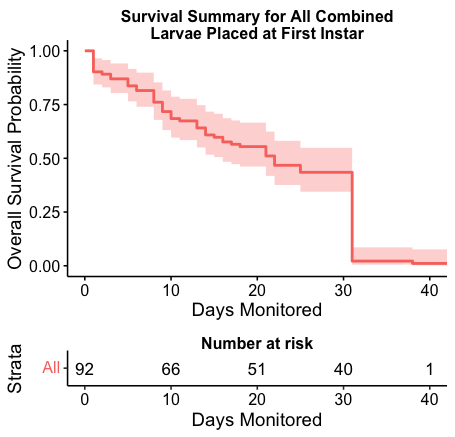
\includegraphics[width=0.5\linewidth]{../Figures/Figure_4} 

}

\caption{Survival analysis results illustrated for all combined larvae: A/B/C at First Instar and Control.}\label{fig:Figure4}
\end{figure}

\begin{figure}

{\centering 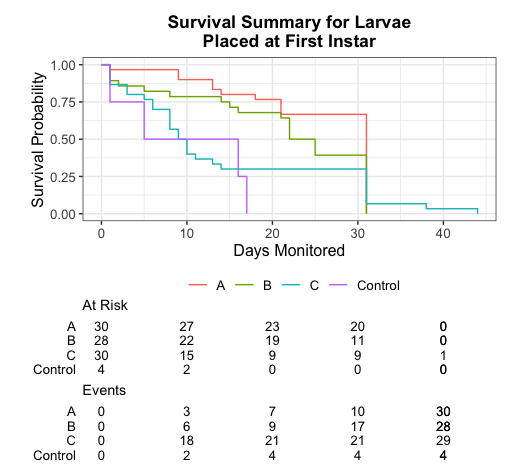
\includegraphics[width=0.5\linewidth]{../Figures/Figure_5} 

}

\caption{Survival analysis results illustrated for each treatment: A/B/C at First Instar and Control.}\label{fig:Figure5}
\end{figure}

I performed a chi-square test comparing treatment group and mortality
(binary event). The resulting chi-squared value is 90.186 on 3 degrees
of freedom with \(p < 2.2e-16\). The p-value is highly significant and
therefore indicates that the two variables of treatment and mortality
are dependent.

\hypertarget{discussion}{%
\section{Discussion}\label{discussion}}

\hypertarget{pupation-2}{%
\subsubsection{Pupation}\label{pupation-2}}

In general, the manipulated diet treatments yielded lower overall
pupation rates (Figure 1), slower pupation time (Table 1), lower pupal
mass (Table 2), and higher mortality rates (Figure 5) compared to the
control treatment. However, this is to be expected since the control
diet is a well-proven formula for rearing laboratory FAW colonies.

When looking at specific differences between A, B, and C treatments, it
seems that a higher carbohydrate content and lower protein is not
conducive to FAW larval success. The C diet (P:C ratio of 1:5) did not
produce any pupae whether started at first instar or third instar, while
the B diet at least had some pupae for both initial age groups and the A
diet had several pupae when started at third instar age. The higher
protein content in the A diet seemed to help more third instar larvae
make it to the pupal stage, but perhaps the too-low carbohydrate content
prevented those started at first instar from surviving that long.

When looking at statistical analysis results for third instar to
pupation, the ANOVA revealed a very low p-value, indicating significant
differences between the means of the treatment groups. Specifically, the
Tukey test showed a large difference between the Control group and A3rd
group and between Control group and B3rd. This demonstrates that the
time to pupation was significantly changed when fed manipulated diets A
or B as compared to standard diet. Meanwhile, there was not a
significant difference between A3rd and B3rd. I interpret this to mean
that individuals started at third instar for both A and B diets took a
similar number of days to reach pupation; however, there were B1st
individuals that were able to survive until pupation unlike A1st, and
there were more A3rd pupae than B3rd. It seems that overall performance
certainly varies between the diet types.

For pupal masses, the ANOVA was significant, suggesting differences in
the mean masses of the treatment groups. However, the Tukey test only
indicated a significant difference between Control and A3rd. T-tests
suggested that Control vs.~B3rd was also significant and that Control
vs.~B1st almost was as well. I believe this partially has something to
do with the low sample sizes for B1st (N = 2 pupae) and B3rd groups (N =
3 pupae) as compared to A3rd (N = 11 pupae) and Control (N = 26 pupae).
Moreover, the equal macronutrient values in the B diet (P:C 1:1) might
have yielded a more ``ideal'' nutritional content for producing pupae
more equal in mass to Southland-fed individuals.

\hypertarget{mortality-2}{%
\subsubsection{Mortality}\label{mortality-2}}

The most larvae overall died on C diet, followed by A diet placed at
first instar. The survival analysis curves show that Control individuals
died pretty early on, perhaps due to being generally unfit, while A and
B individuals gradually died until the age of attempting to pupate,
where they finished dying (noticeable drop in curve on Figure 4 and
Figure 5). C larvae, however, essentially tried to hang on as long as
possible before dying and grew noticeably slower. Very few C larvae
started at third instar made it to the sixth instar, and no larvae
started at first instar made it to the sixth instar, unlike all other
treatments.

The chi-square test for mortality had a highly significant p-value that
indicates dependence between treatment and mortality. This means that
treatment group (A, B, C, or Control) correlated significantly with
mortality rates. Based on the chi-square test and survival analysis
curves, it appears that the ``poorer'' diets took longer to induce
mortality but with higher event numbers (i.e., more died on worse diet),
while ``better'' diets had quicker mortality events in lower numbers.

Given that almost no larvae survived successfully when started on
manipulated diet at first instar, these diet recipes should not be used
for rearing fall armyworms for their whole larval period; however,
considering the differences between development for A, B, and C formulas
overall, there is a clear difference in nutritional composition that is
affecting performance. These artificial diets can still be used to
directly manipulate nutrient intake for future fall armyworm experiments
as long as they are fed during a shorter portion of the lifespan right
before use in experimental tests.

\hypertarget{conclusions-future-directions}{%
\section{Conclusions \& Future
Directions}\label{conclusions-future-directions}}

Manipulation of protein:carbohydrate ratios in artificial diet tends to
result in significant differences in the survival and pupation rates of
fall armyworm larvae compared to a standard diet formula. FAW larvae fed
a standard diet exhibited faster development times and minimal mortality
with very high pupation rates. Manipulated diets caused high levels of
mortality and low rates of (delayed) pupation.

When comparing treatment diets to each other, larvae were more likely to
survive and pupate when protein was higher than carbohydrates, but an
equal ratio of protein:carbohydrates still allowed for some pupation
success. Higher carbohydrate levels were not conducive to survival and
resulted in 100\% mortality. In general, larvae placed on treatment diet
at first instar were unable to pupate, while larvae placed at third
instar (for A and B treatments) were more likely to pupate.

Moving forward, I will be testing how this variation in resource quality
--- along with temperature --- might affect cannibalistic behaviors and,
subsequently, virus transmission in this system. Based on the
information presented here, I consider the treatment diet formulas to be
different enough in nutrition to be used in the next experiment as well.
Given the low survival rates when fed treatment diet from first instar
age, future larvae will be reared on Southland brand diet from neonate
age until early third instar then fed treatment diet for one whole
instar. As an early fourth instar, they will be placed in a small arena
and essentially given the option between a portion of their assigned
artificial diet and an infected conspecific. Larvae will be observed for
cannibalism and then placed back on Southland diet to determine either
virus-related death or successful pupation. It is my prediction that
being fed diet with a higher carbohydrate content relative to protein
(i.e., a more diluted resource) will cause FAW larvae to more readily
cannibalize and become infected more easily. Published research suggests
that warmer temperatures also promote disease transmission and outbreak
intensity in this species \autocite{elderd_warmer_2014}. I am interested
in seeing how this interaction between both temperature variation and
level of resource quality might lead to experimental differences in
cannibalism and virus transmission.

In the face of climate change, it is important to understand the
potential impacts of nutrient dilution and resource quality variation in
insect herbivore species. When considering an agricultural pest as
widespread and invasive as the fall armyworm, it is particularly
beneficial to understand this concept and predict how it may apply to a
field setting.





\newpage
\singlespacing 
\printbibliography[title=Literature Cited]

\end{document}
